%\documentclass[tikz,convert={density=800,outext=.png},border=5pt]{standalone}
\documentclass[preview]{standalone}

\usepackage[utf8]{inputenc} % utf8 encoding
\usepackage{amsmath} % nice math symbols
     
\usepackage{tikz}
\usetikzlibrary{shapes,positioning,calc}

\newcommand{\opredictors}[4]{
	\node[z_pred, minimum width = #2pt, minimum height = #2pt] (z_#1) at ($(#3,#4)$) {};
	\node[z_pred, minimum width = #2, minimum height = #2] at ($(z_#1)+(#2/500.0,-#2/1000.0)$) {};
	\node[z_pred, minimum width = #2, minimum height = #2] at ($(z_#1)+(#2*2/500.0,-#2*2/1000.0)$) {};
	\node (point_#1) at ($(z_#1)+(0,-#2/500)$) {$\cdot$};			
	\node at ($(point_#1)+(#2/1500.0,-#2/1500.0)$) {$\cdot$};
	\node at ($(point_#1)+(#2/750.0,-#2/750.0)$) {$\cdot$};
	\node[z_pred, minimum width = #2, minimum height = #2] (z_l_#1) at ($(z_#1)+(#2/125.0,-#2/250.0)$) {};
	
	\draw[ultra thick, gray!60!black] ($(z_l_#1)+(-3pt,4.5pt)$) -- ($(z_l_#1)+(-3pt,-4.5pt)$);
	\node at (z_l_#1) {$\cdots$};
	\node[font=\small] at ($(z_l_#1)+(-1pt,-3pt)$) { $z_1$};
	\node[font=\small] at ($(z_l_#1)+(1pt,3pt)$) {$z_h$};
	\draw[ultra thick, gray!60!black] ($(z_l_#1)+(3pt,4.5pt)$) -- ($(z_l_#1)+(3pt,-4.5pt)$);
}	

\newcommand{\ppredictors}[4]{
	\node[z_pred, minimum width = #2pt, minimum height = #2pt] (z_#1) at ($(#3,#4)$) {};
	\node[z_pred, minimum width = #2, minimum height = #2] at ($(z_#1)+(#2/500.0,-#2/1000.0)$) {};
	\node[z_pred, minimum width = #2, minimum height = #2] at ($(z_#1)+(#2*2/500.0,-#2*2/1000.0)$) {};
	\node (point_#1) at ($(z_#1)+(0,-#2/500)$) {$\cdot$};			
	\node at ($(point_#1)+(#2/1500.0,-#2/1500.0)$) {$\cdot$};
	\node at ($(point_#1)+(#2/750.0,-#2/750.0)$) {$\cdot$};
	\node[z_pred, minimum width = #2, minimum height = #2] (z_l_#1) at ($(z_#1)+(#2/125.0,-#2/250.0)$) {};
	
	\draw[ultra thick, gray!60!black] ($(z_l_#1)+(-3pt,4.5pt)$) -- ($(z_l_#1)+(-3pt,-4.5pt)$);
	\draw[->] ($(z_l_#1)+(-2.5pt,0)$) to[out=50,in=210] ($(z_l_#1)+(2.5pt,0)$);
	\node[font=\small] at ($(z_l_#1)+(-1pt,-3pt)$) {$z^c$};
	\node[font=\small] at ($(z_l_#1)+(1pt,3pt)$) {$z^e$};
	\draw[ultra thick, gray!60!black] ($(z_l_#1)+(3pt,4.5pt)$) -- ($(z_l_#1)+(3pt,-4.5pt)$);
}	

\begin{document}
	
	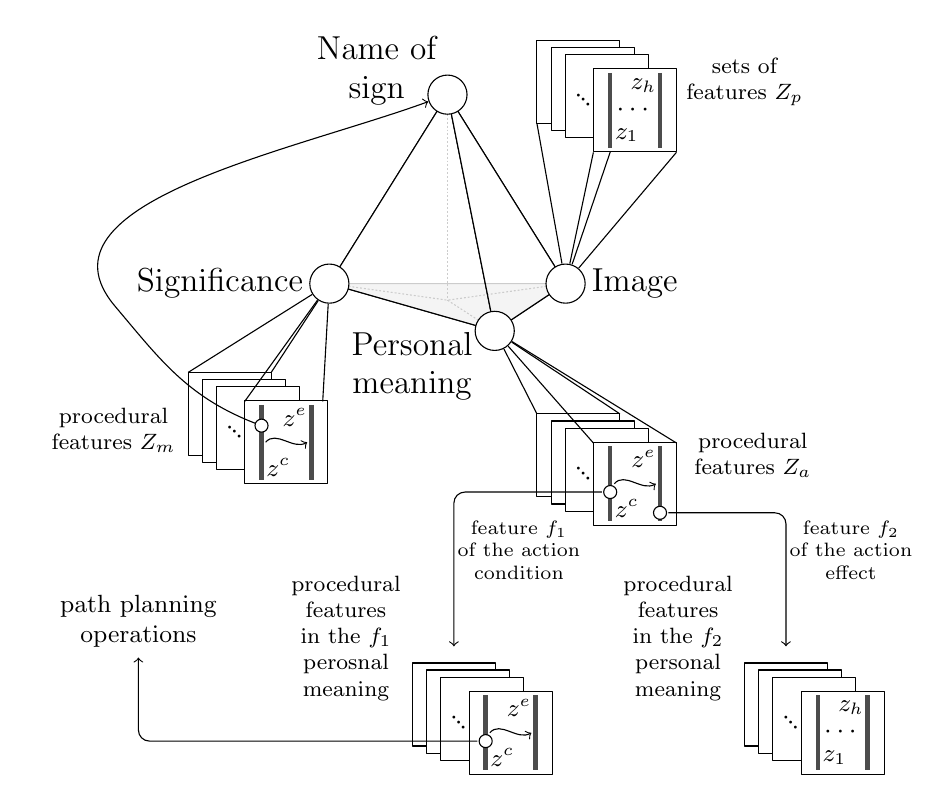
\begin{tikzpicture}[join=round,scale=3.0,node distance = -0.05]
		\tikzstyle{sign_comp}=[draw, circle,fill=white, scale=1.5];
		\tikzstyle{label_small}=[align=center,font=\footnotesize,fill=white,opacity=0.8,text opacity=1];
		\tikzstyle{coord_cine}=[dash pattern=on 0.7 off 0.7];
		
		\tikzstyle{z_pred}=[draw, rectangle,fill=white];


		\filldraw[fill=white] (0.0,0.2) -- (0.5,1.0) -- (1.0,0.2) -- cycle;
		\filldraw[fill=black!20] (0.0,0.2) -- (0.7,0.0) -- (1.0,0.2) -- cycle;
		
		\draw[coord_cine] (0.5,1.0) -- (0.5,0.13);
		\draw[coord_cine] (0.0,0.2) -- (0.5,0.13);
		\draw[coord_cine] (0.7,0.0) -- (0.5,0.13);
		\draw[coord_cine] (1.0,0.2) -- (0.5,0.13);
		
		\filldraw[fill=white,fill opacity=0.8] (0.0,0.2) -- (0.5,1.0) -- (0.7,0.0) -- cycle;
		\filldraw[fill=white,fill opacity=0.8] (0.7,0.0) -- (0.5,1.0) -- (1.0,0.2) -- cycle;
		
		\node[sign_comp] (s_m) at (0.0,0.2) {};
		\node[sign_comp] (s_p) at (1.0,0.2) {};
		\node[sign_comp] (s_n) at (0.5,1.0) {};
		\node[sign_comp] (s_a) at (0.7,0.0) {};
		\node[left = of s_m, font=\large] {Significance};
		\node[right = of s_p, font=\large]{Image};
		\node[align=center, font=\large] at ($(s_n)+(-0.30,0.1)$) {Name of\\sign};
		\node[align=center, font=\large] at ($(s_a)+(-0.35,-0.15)$) {Personal\\meaning};		
		

		\ppredictors{m}{30}{-12pt}{-10pt}		
		\draw[thin] (-7pt,-5pt) -- (s_m);
		\draw[thin] (-17pt,-5pt) -- (s_m);
		\draw[thin] (-0.8pt,-8.5pt)  -- (s_m);
		\draw[thin] (-10.2pt,-8.5pt) -- (s_m);
		\node[align=center,font=\footnotesize] at (-26pt,-12pt) {procedural\\features $Z_m$};		
		
		\draw[thin] (35pt,25pt) -- (s_p);
		\draw[thin] (25pt,25pt) -- (s_p);
		\draw[thin] (41.8pt,21.5pt)  -- (s_p);
		\draw[thin] (31.8pt,21.5pt) -- (s_p);
		\opredictors{p}{30}{30pt}{30pt}		
		\node[align=center,font=\footnotesize] at (50pt,30pt) {sets of\\features $Z_p$};
		

		\ppredictors{a}{30}{30pt}{-15pt}	
		\draw[thin] (35pt,-10pt) -- (s_a);
		\draw[thin] (25pt,-10pt) -- (s_a);
		\draw[thin] (41.8pt,-13.5pt)  -- (s_a);
		\draw[thin] (31.8pt,-13.5pt) -- (s_a);	
		\node[align=center,font=\footnotesize] at (51pt,-15pt) {procedural\\features $Z_a$};		
		
		\opredictors{a1}{30}{55pt}{-45pt}
		
		\ppredictors{a2}{30}{15pt}{-45pt}
		\draw[->,rounded corners] ($(z_l_a)+(-4pt,-1pt)$) -- ($(z_l_a)+(-10pt,-1pt)$) -| ($(z_a2)+(0,7pt)$);
		\node[draw, circle, fill=white, scale=0.5] at ($(z_l_a)+(-3pt,-1pt)$) {};
		\draw[->,rounded corners] ($(z_l_a)+(4pt,-3.5pt)$) -- ($(z_l_a)+(10pt,-3.5pt)$) -| ($(z_a1)+(0,7pt)$);
		\node[align=center,font=\scriptsize] at ($(z_l_a)+(26pt,-8pt)$) {feature $f_2$\\of the action\\effect};
		\node[align=center,font=\scriptsize] at ($(z_l_a)+(-14pt,-8pt)$) {feature $f_1$\\of the action\\condition};
		\node[draw, circle, fill=white, scale=0.5] at ($(z_l_a)+(3pt,-3.5pt)$) {};
		
		\node[align=center,font=\small] (ppo) at (-23pt,-35pt) {path planning\\operations};
		\draw[->,rounded corners] ($(z_l_a2)+(-4pt,-1pt)$) -| (ppo.south);
		\node[draw, circle, fill=white, scale=0.5] at ($(z_l_a2)+(-3pt,-1pt)$) {};
		
		\node[align=center,font=\footnotesize] at (2
		pt,-37pt) {procedural\\features\\in the $f_1$\\perosnal\\meaning};
		\node[align=center,font=\footnotesize] at (42pt,-37pt) {procedural\\features\\in the $f_2$\\personal\\meaning};
		
		\draw[->,rounded corners] ($(z_l_m)+(-3pt,2pt)$) to[out=160,in=-50](-25pt,2pt) to[out=130,in=200] (s_n);
		\node[draw, circle, fill=white, scale=0.5] at ($(z_l_m)+(-3pt,2pt)$) {};
	\end{tikzpicture}


\end{document}